\chapter{Introduction}
\graphicspath{{./Introduction/img/}}

Nowadays image processing is being used in many applications like improvements in
photography, recognizing parts and their arrangement in industry applications, 
face-recognition in photos or to scan objects with 3D cameras for creating
models of them.

Recently Microsoft startet to ship the Kinect camera, which was ment to enable
gamers of the XBox-360 to control their in-game avatar with their own body.
As soon it was released a contest was proclaimed to write a free driver to make it a
usable on different systems, like Linux or Windows.

Today the Kinect is also used in WillowGarages Robot Operating System,
where it can act as cheap laser scanner for their Turtlebot. The Turtlebot 
(/url{www.turtlebot.org}) was designed to give home users who are interested in 
robotics the opportunity to experiment with robotics on their own.

\begin{figure}[htp]
\begin{center}
  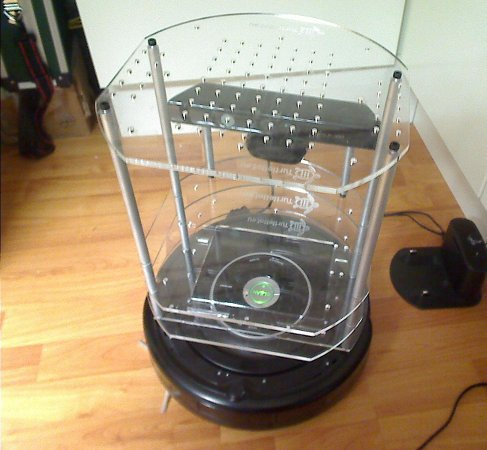
\includegraphics[width=\textwidth/3]{turtlebot.jpg}
  \caption{Turtlebot EU-Version}
  \label{figure:turtlebot}
\end{center}
\end{figure}

This thesis will have a look on the data characteristics and the accuracy of the
Kinect camera and use the results to find surfaces arranged to the camera and to 
recognize different signs on them with pattern matching in the corresponding regions
in the RGB picture. The basic idea behind is to speed up the template Matching 
by only searching interesting regions of the color picture, regions which are not
suitable in size can be skipped automatically.

\chapter{Basics}

\section{Robot Operating System (ROS)}
  
\begin{figure}[htp]
	\centering
	
\includegraphics[scale=2]{ROS_LOGO.pdf}
	\caption{ROS Logo}
\end{figure} 

The Robot Operating System or short ROS is a meta operating system from WillowGarage, which is designed for usage with distributed 
robot systems. It's called a meta operating system because it needs another operating system to run. It's mainly developed for Ubuntu 
(a Linux distribution) but it also supports other Operating Systems like Windows and Mac OS, but the support for them can still be considered 
as experimental. 

It also works together with a Google Android device by runnning a special software which makes the device available
as hardware extension, enabling processes on different machines to access cameras, accelerometers and the display.
The basic underlying principle of ROS is the Publisher Subscriber Pattern further called PSP, it's a pattern which 
implements the realworld behaviour of publishers and subscribers (e.g. newspaper) in software. 
The publishing house advertises and publishes its newspaper or magazine while the subscribers look at the advertisements
and subscribe to the newspaper like seen in figure \vref{figure:psp_real}.

\begin{figure}[htp]
	\centering
	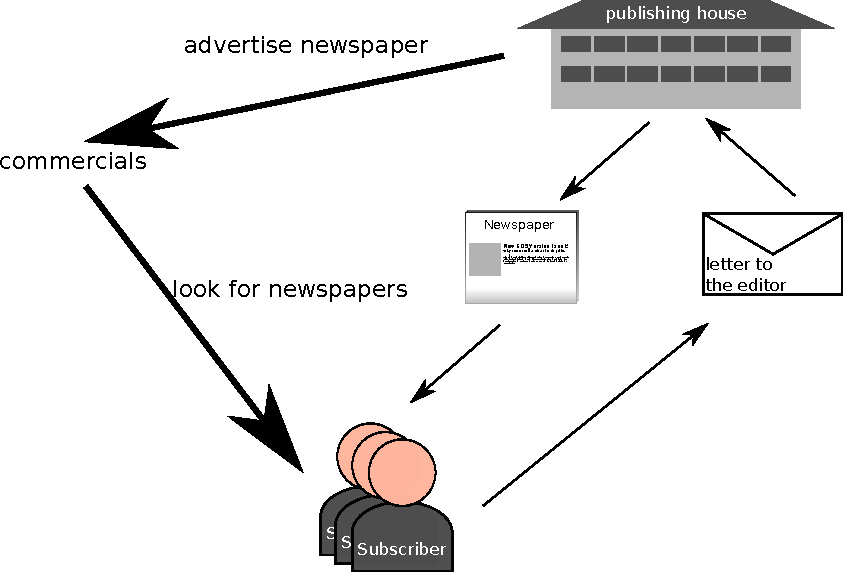
\includegraphics[scale=0.7]{PS_Newspaper.pdf}
	\caption{Publisher Subscriber Priciple in Reality}
	\label{figure:psp_real}
\end{figure} 


In the PSP the newspapers are now called topics. A PSP system is a subset of different applications, those applications are called nodes.  
Each node can publish or subscribe multiple topics at the same time. So it is possible to create a network of different nodes, which
do processing or act as user interface. The advertisements of the real world are replaced by a so called master. 
The master knows everything about the communication channels, all nodes, the computer they run on and 
which topics they subscribe and publish to. When a new node starts up, it checks for other nodes publishing or subscribing the relevant topics
and connects with them. An example of this is shown in figure \vref{figure:psp_ROS}.
In the picture there are different nodes for the robots running gear, its laserscanner, the motion planing system and the graphical user interface.
connected together by topics.

\begin{figure}[htp]
	\centering
	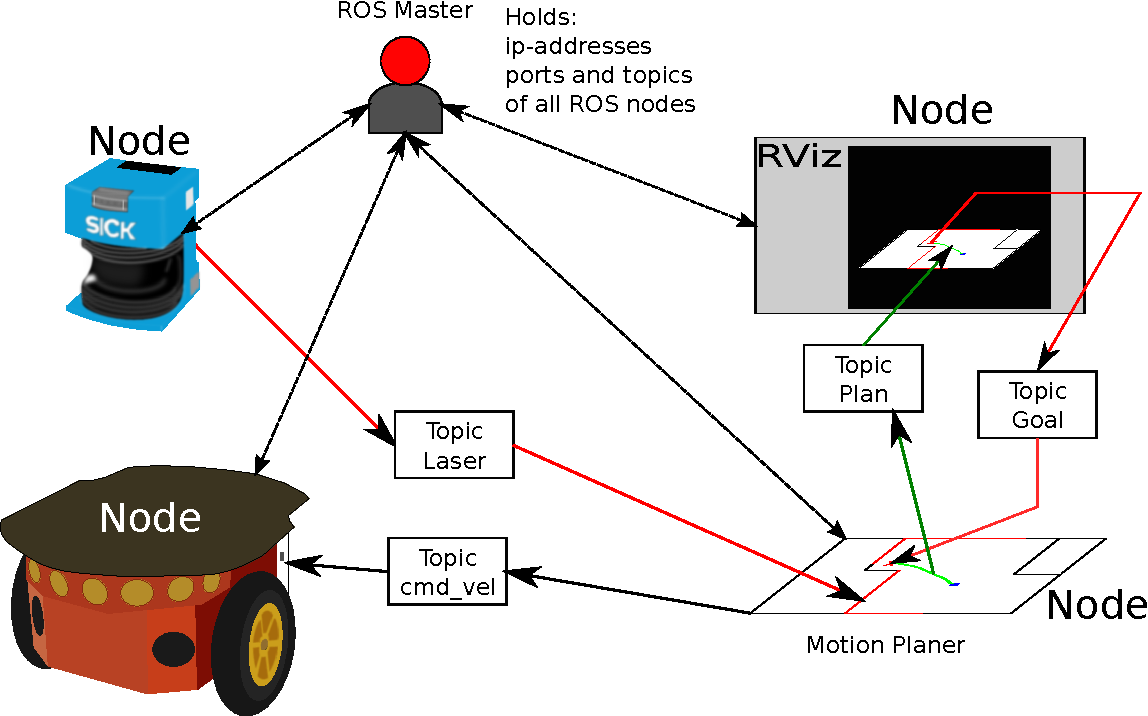
\includegraphics[scale=0.6]{PS_ROS.pdf}
	\caption{Publisher Subscriber Pattern in ROS}
	\label{figure:psp_ROS}
\end{figure} 

In this work the output of the rViz-node (short form for robot visualizer) will be used to display changes to the depth- and 
rgb-image of the Kinect. rViz is a tool to display various informations like video streams, maps, paths, positions and the
so called point cloud.
\clearpage

\section{Point Cloud}
The point cloud is data set which contains the three dimensional position for each pixel of a 3D camera. 
If available, it can also contain the color or grayscale values of each pixel. 
The point cloud data can be collected from a stereo camera, a laser scanner which rotates around an axis or 
from cameras like the Microsoft Kinect.

\begin{figure}[htp]
	\centering
	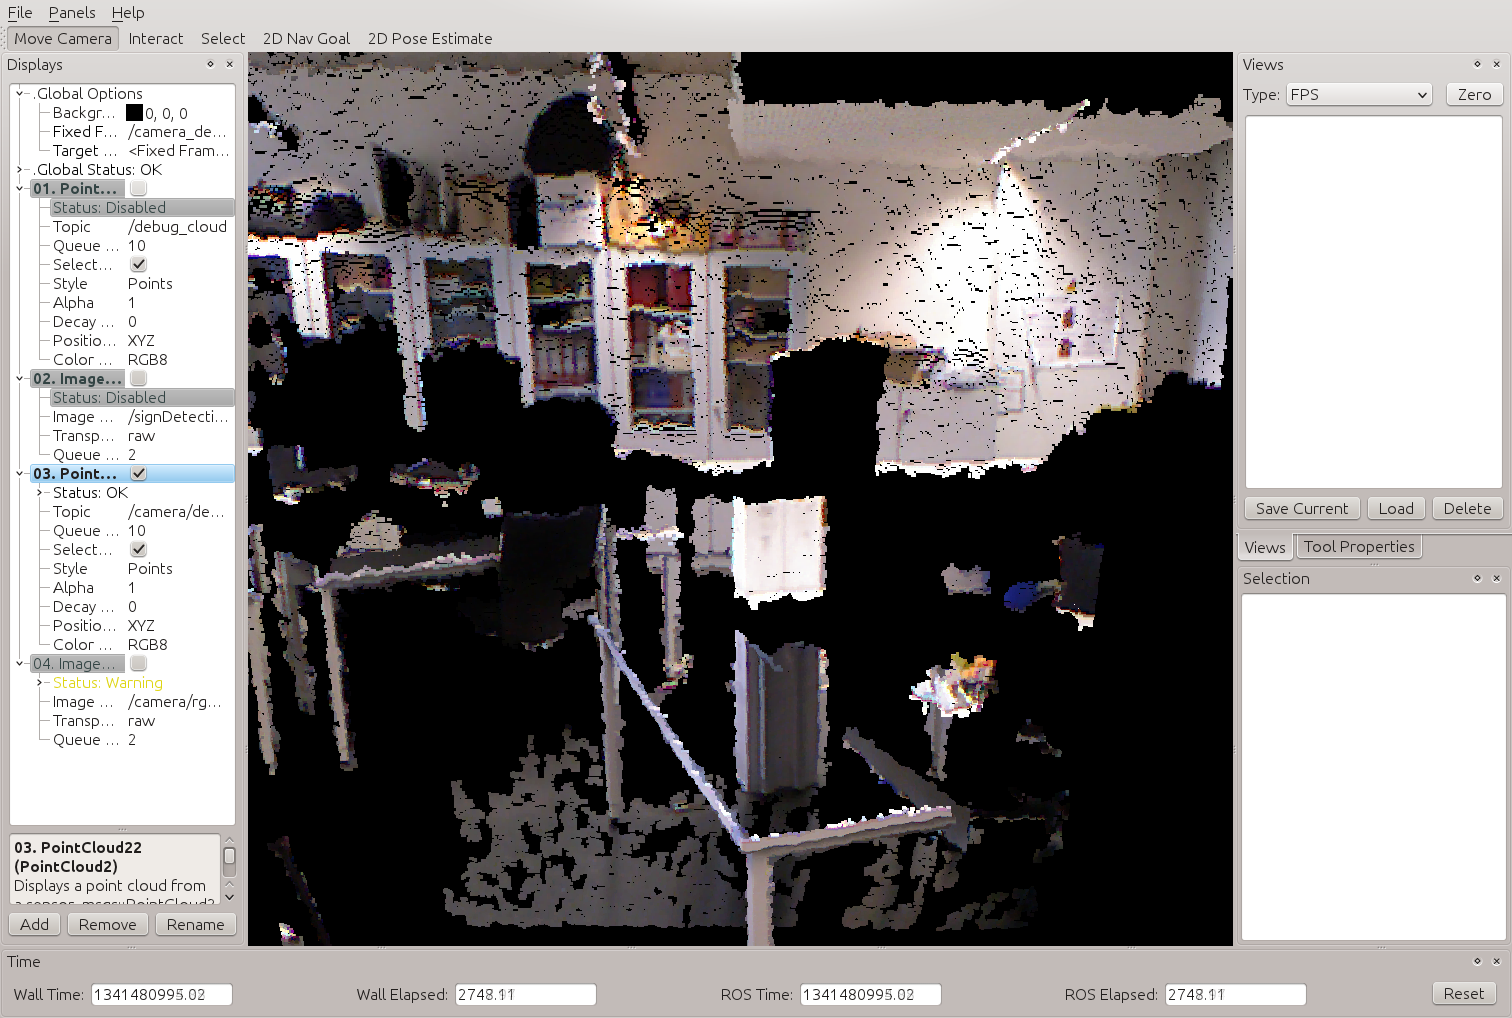
\includegraphics[width=\textwidth]{RVizPointCloud.png}
	\caption{Robot Visualizer displaying the Point Cloud}
	\label{figure:RVizPointCloud.png}
\end{figure}
\clearpage

\section{OpenCV}

The Open Source Computer Vision Library (OpenCV) is an open computer vision and machine learning software library. OpenCV was built to provide a common infrastructure for vision applications and to accelerate the use of machine perception in the commercial products. To enable this, OpenCV has a BSD license to make it easy for businesses to use and modify the code.

The library has more than 2500 optimized algorithms. OpenCV contains a comprehensive set of both classic and state of the art computer vision and machine learning algorithms. These algorithms can be used, for example, to detect and recognize faces, identify objects, classify human actions in videos, track camera movements, track moving objects, extract 3D models of objects, produce 3D point clouds from stereo cameras, stitch images together to produce a high resolution image of an entire scene, find similar images from an image database, remove red eye from images taken using flash, follow eye movements, recognize scenes and establish markers to overlay the scenes with augmented reality to name a few. OpenCV has well over 5 million downloads, has an active user group with over 47 thousands registered members. OpenCV is used extensively in companies, research groups and by governmental bodies.

Some well known companies that use OpenCV are Google, Yahoo, Microsoft, Intel, IBM, Sony, Honda, Toyota. Many startups such as Applied Minds, VideoSurf, and Zeitera make extensive use of OpenCV. OpenCV’s deployed uses span the range from stitching streetview images together, detecting intrusions in surveillance video in Israel, monitoring mine equipment in China, helping robots navigate and pick up objects at Willow Garage, detection swimming pool drowning events in Europe, running interactive art in Spain and New York, checking run ways for derbies in Turkey, inspecting labels on products in factories around the world on to rapid face detection in Japan.

It runs on Windows, Linux, Mac, Android and has C++, C, Python and Java (Android only) interfaces. OpenCV leans mostly towards real-time vision applications and takes advantage of MMX and SSE instructions when available. A CUDA interface is being developed right now. There are over 500 algorithms and about 10 times as many functions that compose or support those algorithms. OpenCV is written natively in C++ and has a templated interface that works seamlessly with std containers. Its native data type is a general matrix class that reference counts and leverages EIGEN.
\cite{willowgarage:opencv}
\clearpage

\section{Kinect}
\begin{figure}[htp]
	\centering
	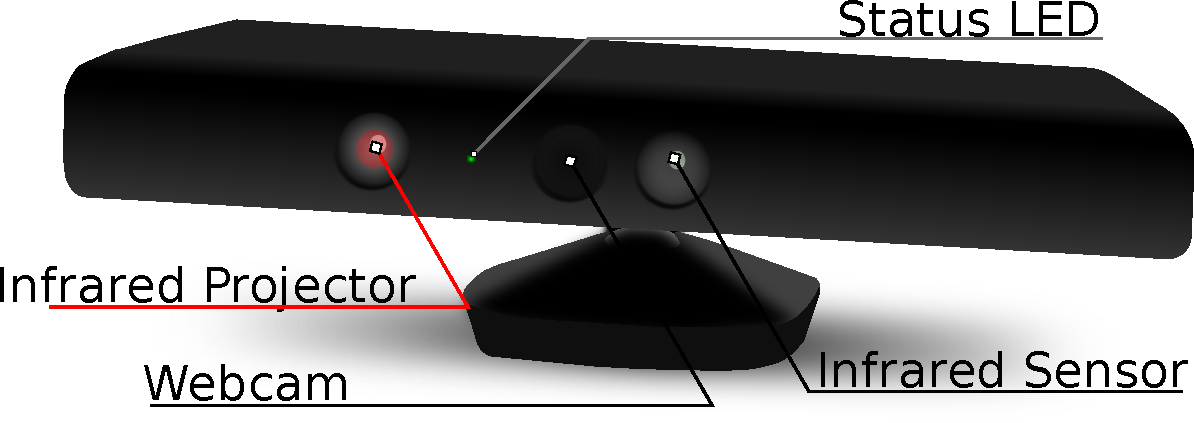
\includegraphics[scale=0.7]{Kinect.pdf}
	\caption{Microsoft Kinect Camera Overview}
	\label{figure:kinect_camera}
\end{figure}

The Kinect is a combination of a standard color camera and a depth sensor produced by Microsoft, a so called RGB-D camera. 
The depth sensor is produced by Primesense and it's working principle is currently a secret of the manufacturer. 
The known facts are, that the Kinect uses an ir-projector to draw a grid of very small points onto each surface 
(see figure \vref{figure:kinect_camera}) and an ir-camera to process the result somehow.  
There are different approaches on how it might work, the most resonable approach is that it uses 
specific groups of points and their position on the resulting camera image to calculate how far 
away they are. This is the same way a laser scanner works. 
It sends out a laser beam and the sensor is aranged in a different viewing angle than the beam.
If the beam now hits a surface its position in the camera picture relates to the distance of the surface.
(see in figure \vref{figure:ls_WP}). This it would be the same for the Kinect points but in 3 dimensions 
(see in figure \vref{figure:kinect_WP}).

ASUS is also offering cameras with the Primesense chipset for developers, the XTion Pro and the XTion Pro Live.
The difference between those cameras is, that the XTion Pro does not include a webcam.

In the recent past Microsoft created a new PC version of the Kinect, which is called Kinect for Windows.
This camera offers a greater viewing angle, while being able to detect objects closer to the camera.
The problem of objects being to close will be discussed later in this document.

\begin{figure}[htp]
	\centering
	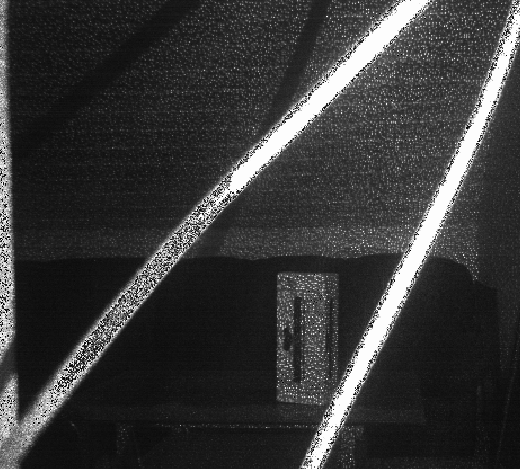
\includegraphics[scale=1]{ir_kinect.png}
	\caption{Kinect IR Sensor Image}
	\label{figure:kinect_ir}
\end{figure}

\begin{figure}[htp]
	\centering
	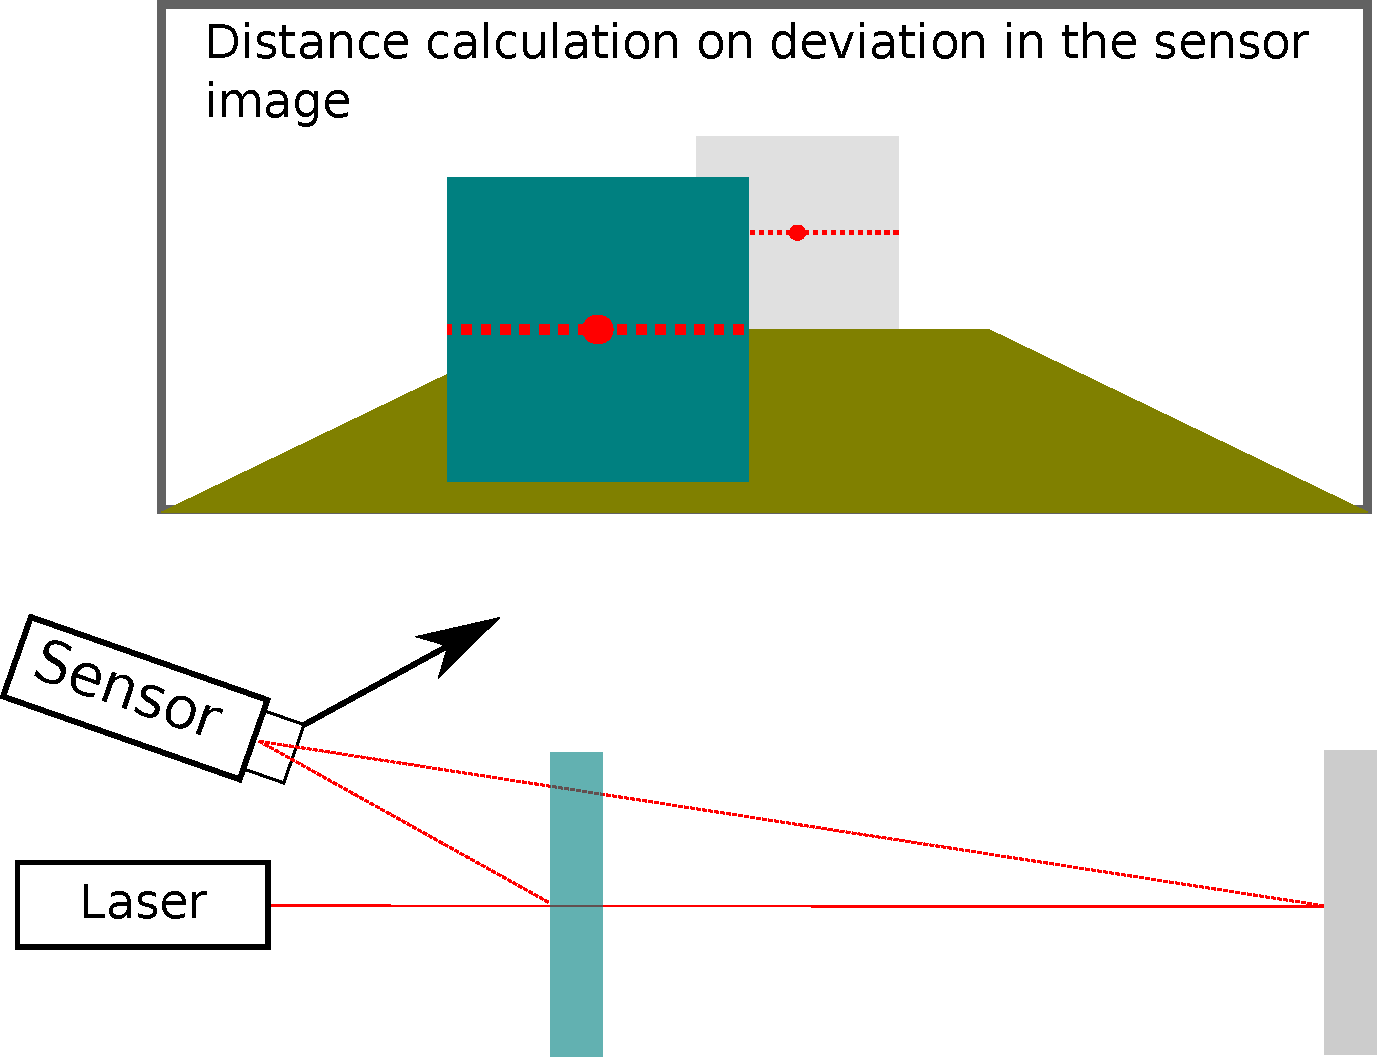
\includegraphics[scale=0.5]{laserScannerPrinciple.pdf}
	\caption{Laser Scanner Working Principle}
	\label{figure:ls_WP}
\end{figure}


\begin{figure}[htp]
	\centering
	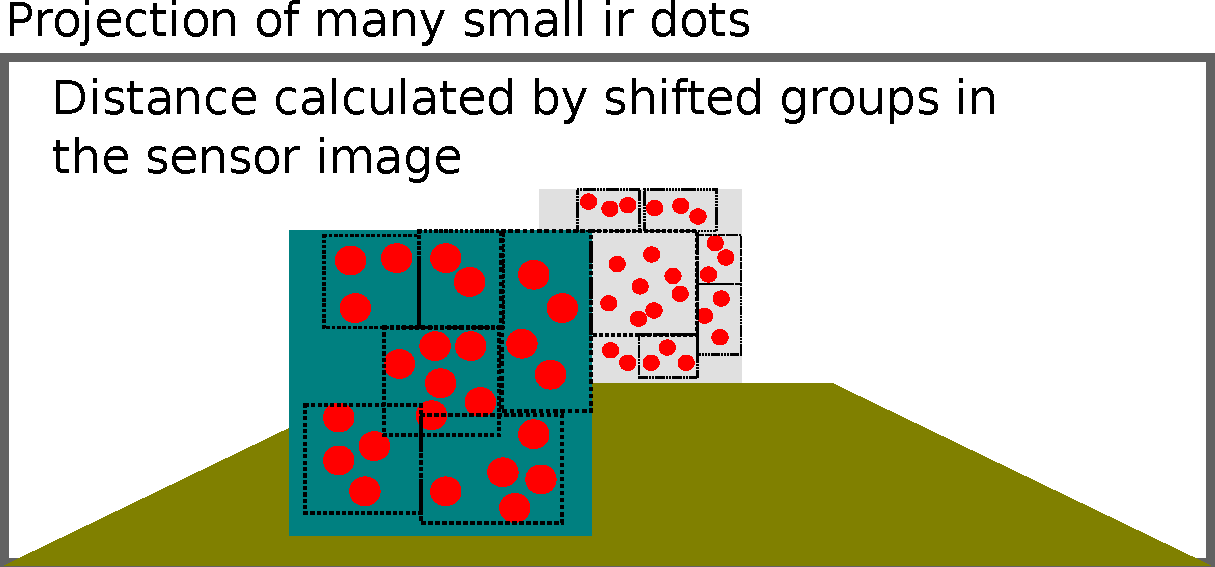
\includegraphics[scale=0.5]{kinect_principle.pdf}
	\caption{Kinect Working Principle}
	\label{figure:kinect_WP} 
\end{figure}
\clearpage

\section{OpenNi}

About the OpenNI organization
The OpenNI organization is an industry-led, not-for-profit organization formed to certify and 
promote the compatibility and interoperability of Natural Interaction devices, applications and middleware. 
One of the OpenNI organization goals is to accelerate the introduction of Natural Interaction applications into 
the marketplace.

The founding members of the OpenNI organization are:
\begin{itemize}
  \item PrimeSense, industry leader in Natural Interaction and 3D depth sensing solutions   
  \item Willow Garage, experts in personal robotics applications  
  \item Side-Kick, a leading production house for motion control games  
  \item ASUS joins the OpenNI organization as an industry member providing hardware for purchase to promote Natural Interaction applications
  \item AppSide is the first end-to-end content marketplace for motion-controlled entertainment devices. 
\end{itemize}
\cite{openni:about} 

\section{Mobile Robots Pioneer 3dx}
The Pioneer 3dx is a Research Robot created by Mobile Robots.
\\
\url{http://www.mobilerobots.com/ResearchRobots/PioneerP3DX.aspx}
\\
With its two motored wheels and its stabilization wheel the robot is a so called point robot. That means it's able to 
rotate around its center like a tank which makes path planing and movement a lot easier. 
The robot features a internal microcontroller board which can be remote controlled from an external computing system, 
ultra-sonic distance sensors and bumpers. The robot of the University of Applied Sciences Aalen 
is additionally equipped with a LMS-200 laser scanner from SICK Sensor Technologies, which works
like described in the last chapter.


\begin{figure}[htp]
\begin{center}
  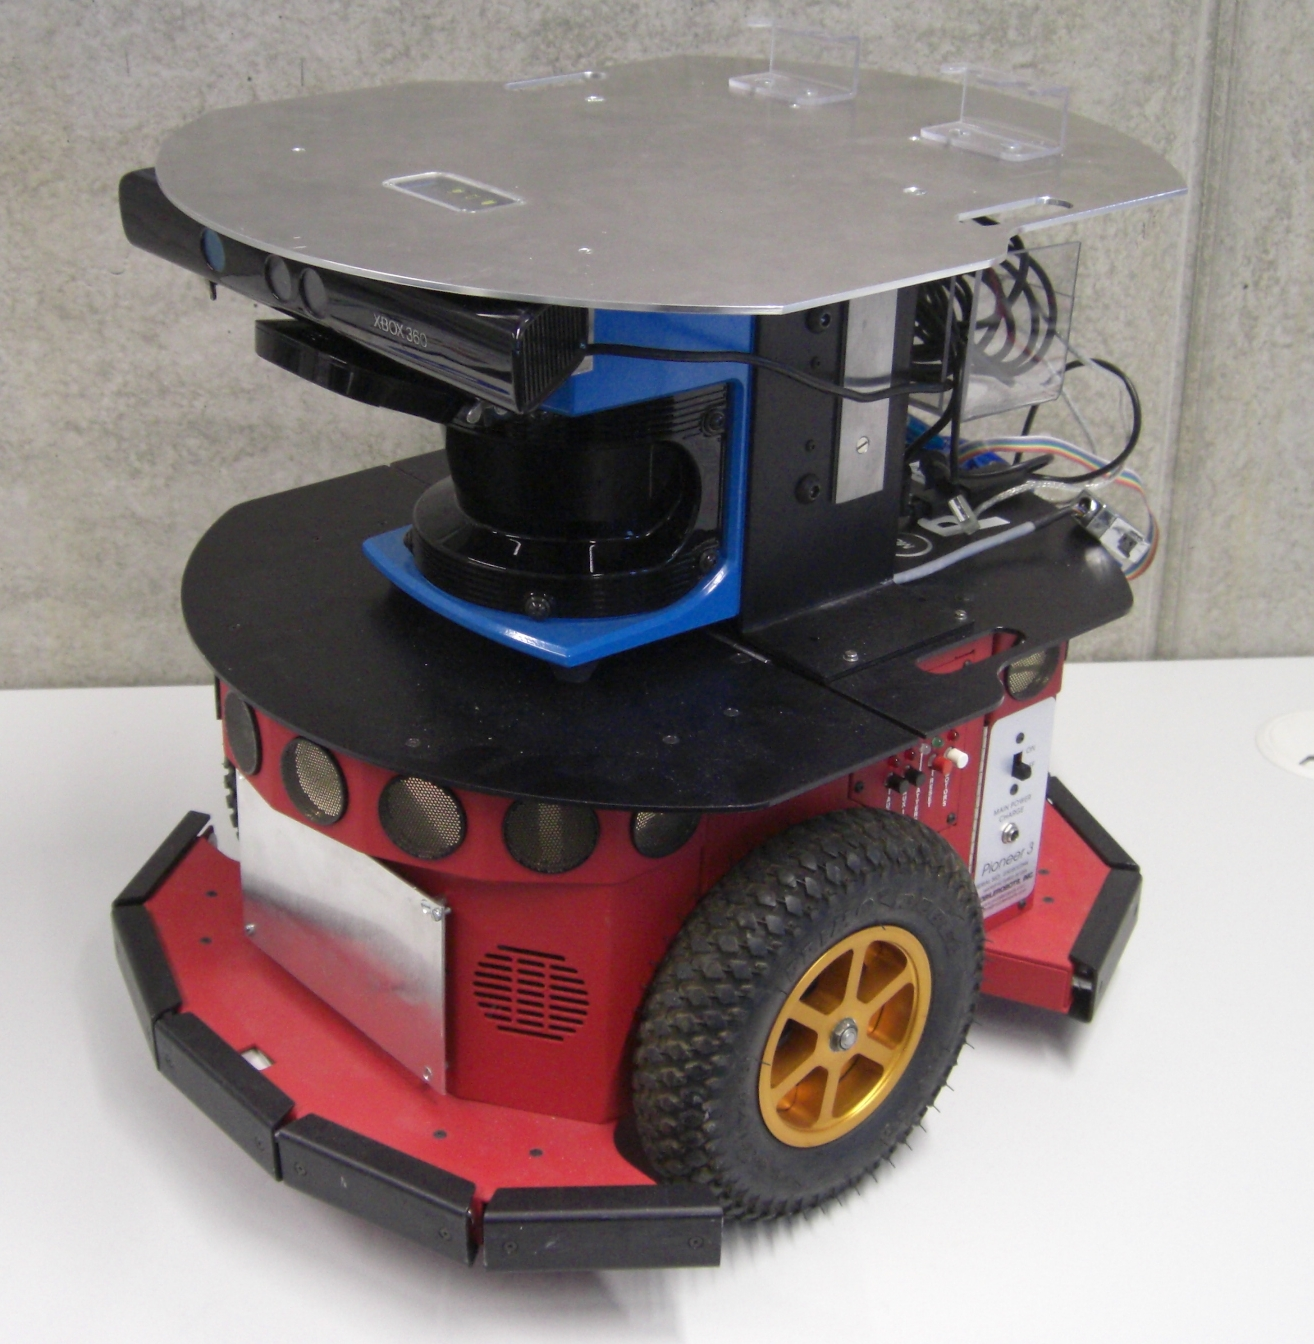
\includegraphics[height=\textheight/3]{pioneer.JPG}
  \caption{Pioneer 3DX}
  \label{figure:Pioneer}
\end{center}
\end{figure}




 

 
